\documentclass{beamer}
%%%%%% UNOFFICIAL ICL BEAMER TEMPLATE V.0.1 %%%%%%
% This is a basic LaTeX Beamer template that I customised to have the logo of ICL and a background picture. Mind that this is NOT an official ICL template but it may still be useful for informal presentations.
% The official ICL graphical identity resources can be found here: http://www3.imperial.ac.uk/graphicidentity
% Please drop me an e-mail or comment via Twitter @AJunyentFerre if you found this was useful or have any suggestion to improve it.
%%%%%%

\usepackage[english]{babel}

%%%%%% THE FOLLOWING FILE CONTAINS THE STYLE DEFINITIONS %%%%%%
\usepackage[utf8]{inputenc}

\definecolor{gris}{rgb}{0.92,0.92,0.92}
\definecolor{blau-upc}{rgb}{.192,.365,.506}

\setbeamercolor{titlelike}{fg=blau-upc}
% \setbeamercolor{barra}{bg=white,fg=white}
\setbeamercolor{capcalera}{bg=blau-upc,fg=white}
\setbeamercolor{section in toc}{fg=blau-upc}
\setbeamertemplate{sections/subsections in toc}[circle]
\setbeamertemplate{itemize items}[circle]
\setbeamercolor{item}{fg=blau-upc}
\setbeamertemplate{blocks}[rounded][shadow=true]
\setbeamercolor*{block body}{bg=gris}
\setbeamerfont{block body}{size=\footnotesize}
\setbeamercolor*{block title}{parent=structure,bg=blau-upc,fg=white}

\setbeamersize{text margin left=12mm,text margin right=12mm}
\setbeamertemplate{navigation symbols}{}

\defbeamertemplate*{headline}{infolines theme}
{
	\begin{beamercolorbox}[wd=\paperwidth,ht=9.5mm,right]{white}%
		
\includegraphics[height=8mm]{./logotips/imperiallogo.pdf}\hspace*{1mm}\vskip0.2ex
	\end{beamercolorbox}
% 	\begin{beamercolorbox}[wd=\paperwidth,ht=0.5mm,left]{barra}%
% 		\hspace*{1mm}
% 	\end{beamercolorbox}
}

\setbeamertemplate{footline}
{
	\hbox{
	\begin{beamercolorbox}[wd=0.1\paperwidth,ht=10mm,left]{}
% 		\hspace*{1ex}
\includegraphics[height=8mm]{./logotips/imperiallogo.pdf}\vskip 2ex
	\end{beamercolorbox}
	\begin{beamercolorbox}[wd=0.8\paperwidth,ht=3ex,center]{}
		\hspace*{4ex}\insertsection\vskip 4ex
	\end{beamercolorbox}
	\begin{beamercolorbox}[wd=0.1\paperwidth,ht=3ex,right]{}
		\insertpagenumber\hspace*{6ex}\vskip 4ex
	\end{beamercolorbox}
	}
}

\setbeamertemplate{title page}
{
	\vbox{}
	\vfill
	\begin{centering}
		{\usebeamerfont{title}\usebeamercolor[fg]{title}\inserttitle}
		\vskip0.2em
		{\usebeamerfont{subtitle}\usebeamercolor[fg]{subtitle}\insertsubtitle}
		\vskip2em\par
		\small\insertauthor\par
		\vskip0.7em\par
		\tiny\insertdate\vskip1em\par
	\end{centering}
% 	\vfill
}

\usebackgroundtemplate{\put(-50,-340){
\includegraphics[width=10cm]{./logotips/imperialback.png}}} 
%%%%%%

%%%%%% TITLE, AUTHOR, DATE DEFINITIONS %%%%%%
\title{Introduction to NGS data}
\subtitle{{\it Principles of genotype and SNP calling\\ and estimation of allele frequencies}}
\author{Matteo Fumagalli}
\date{$22^{nd}$ August 2017}
%%%%%%

\begin{document}

\frame{\titlepage} 

%%%%%%%%%%%%%%%%%%%%%%%%%%%%%%%%%%%%%%%%%%%%%%%%%%%%%%

\frame{

	\begin{figure}
		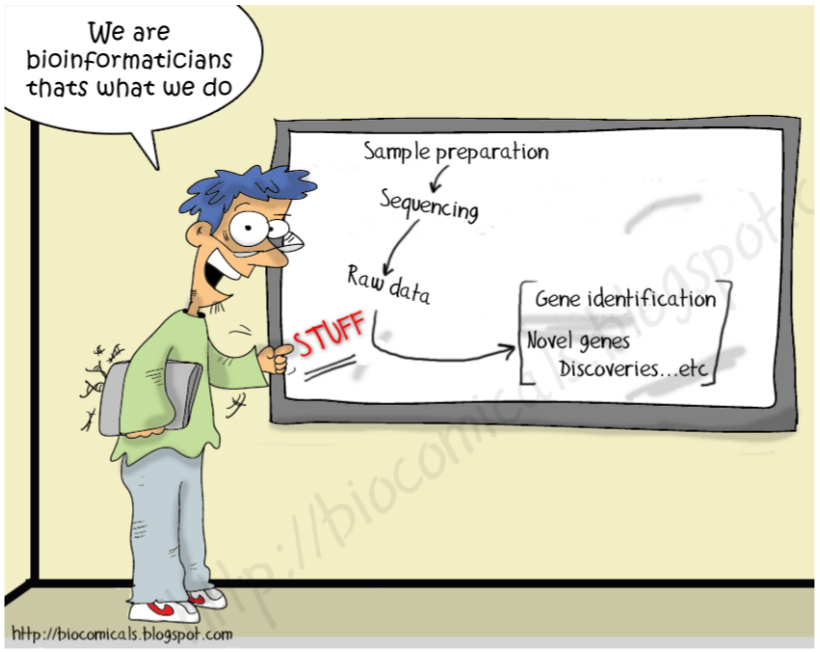
\includegraphics[scale=0.35]{Pics/bioinfo}
	\end{figure}

}

%%%%%%%%%%%%%%%%%%%%%%%%%%%%%%%%%%%%%%%%%%%%%%%%%%%%%%

\frame{\frametitle{Presentation outline}\tableofcontents}

%\section{Introduction}

%\section{Genotype likelihoods}

%\section{Genotype calling}

%\section{Estimation of allele frequencies}

%\section{SNP calling}

%%%%%%%%%%%%%%%%%%%%%%%%%%%%%%%%%%%%%%%%%%%%%%%%%%%%%%

\section{Introduction}

%%%%%%%%%%%%%%%%%%%%%%%%%%%%%%%%%%%%%%%%%%%%%%%%%%%%%%

\frame{\frametitle{Sanger sequencing}

aka first/former generation sequencing

\begin{columns}

	\column{0.3\textwidth}

		\begin{figure}
			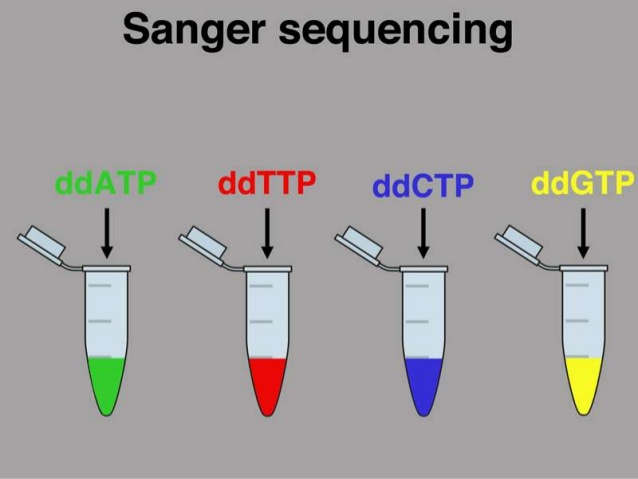
\includegraphics[scale=0.15]{Pics/sanger}
		\end{figure}

	\column{0.7\textwidth}

		\begin{figure}
			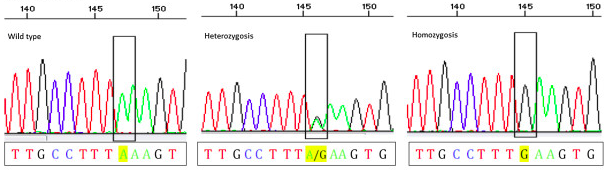
\includegraphics[scale=0.4]{Pics/sangerElectro}
		\end{figure}

\end{columns}

}

%%%%%%%%%%%%%%%%%%%%%%%%%%%%%%%%%%%%%%%%%%%%%%%%%%%%%%

\frame{\frametitle{Next Generation Sequencing}

	\begin{figure}
		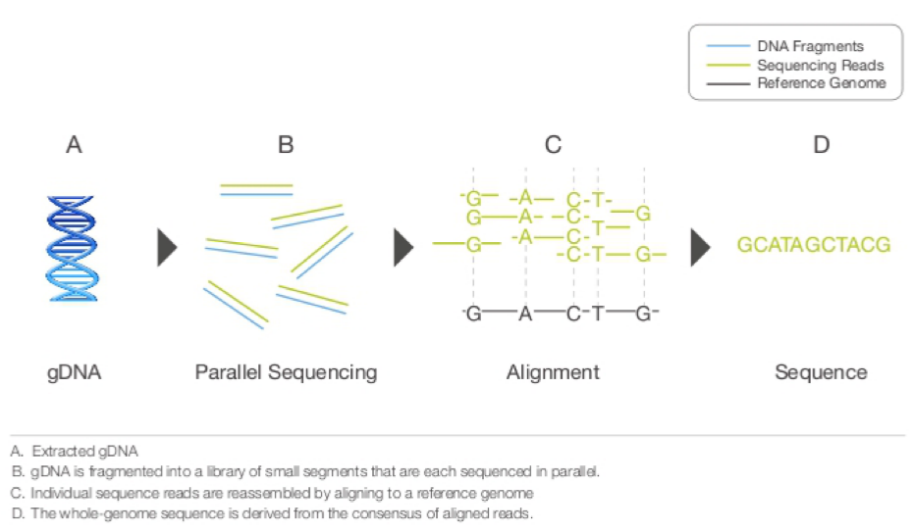
\includegraphics[scale=0.3]{Pics/illumina}
	\end{figure}

}

%%%%%%%%%%%%%%%%%%%%%%%%%%%%%%%%%%%%%%%%%%%%%%%%%%%%%%

\frame{\frametitle{From genomes to variants}

	\begin{figure}
		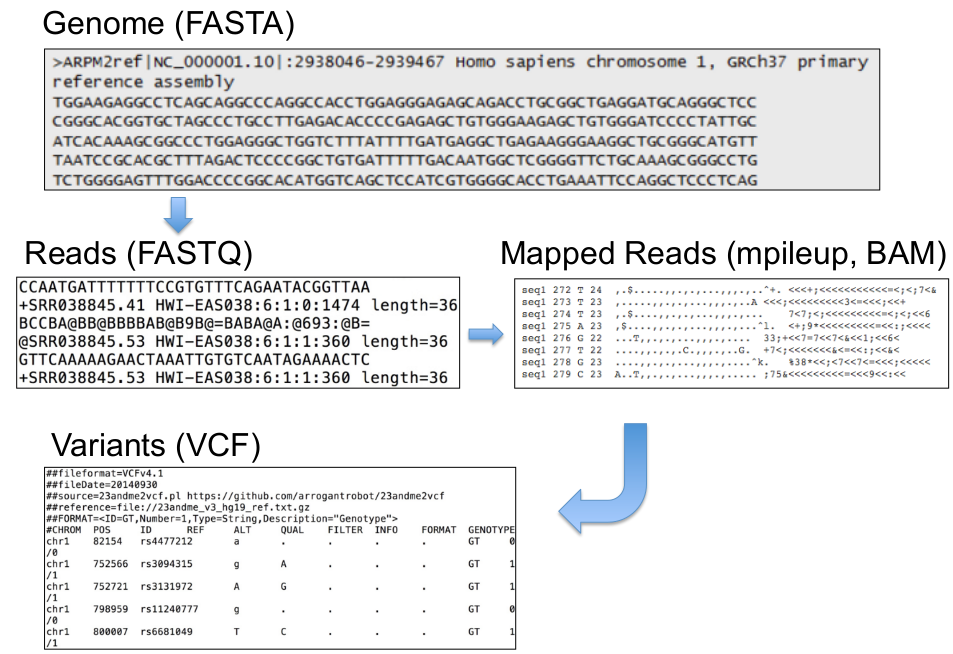
\includegraphics[scale=0.3]{Pics/files}
	\end{figure}

}

%%%%%%%%%%%%%%%%%%%%%%%%%%%%%%%%%%%%%%%%%%%%%%%%%%

\frame{\frametitle{Statistical inference}

	\begin{figure}
		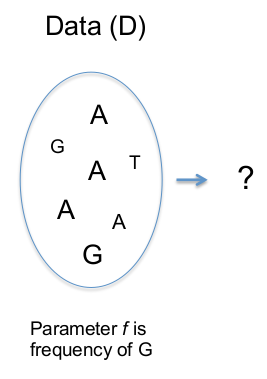
\includegraphics[scale=0.3]{Pics/stat1}
	\end{figure}

}

%%%%%%%%%%%%%%%%%%%%%%%%%%%%%%%%%%%%%%%%%%%%%%%%%%

\frame{\frametitle{Statistical inference}

	\begin{figure}
		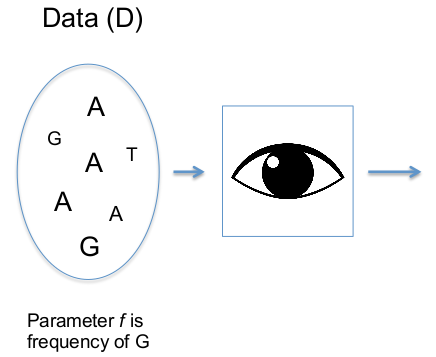
\includegraphics[scale=0.3]{Pics/stat2}
	\end{figure}

}

%%%%%%%%%%%%%%%%%%%%%%%%%%%%%%%%%%%%%%%%%%%%%%%%%%

\frame{\frametitle{Statistical inference}

	\begin{figure}
		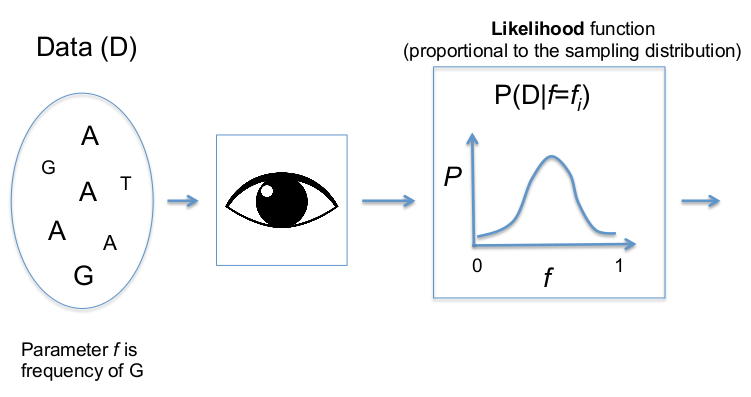
\includegraphics[scale=0.3]{Pics/stat3}
	\end{figure}

}

%%%%%%%%%%%%%%%%%%%%%%%%%%%%%%%%%%%%%%%%%%%%%%%%%%

\frame{\frametitle{Statistical inference}

	\begin{figure}
		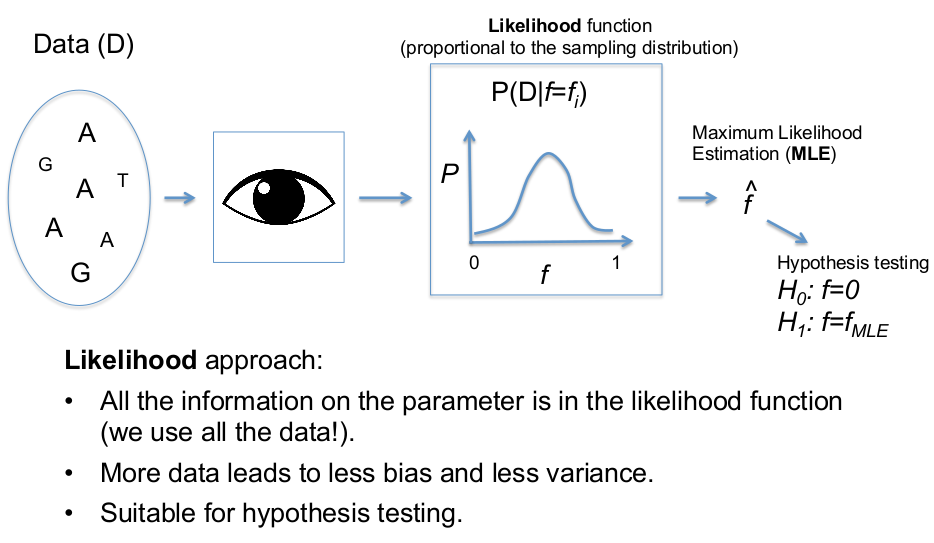
\includegraphics[scale=0.3]{Pics/stat4}
	\end{figure}

}



% Genotype likelihoods

\section{Genotype likelihoods}

%%%%%%%%%%%%%%%%%%%%%%%%%%%%%%%%%%%%%%%%%%%%%%%%%
 
\frame{\frametitle{The data}

	\begin{figure}
		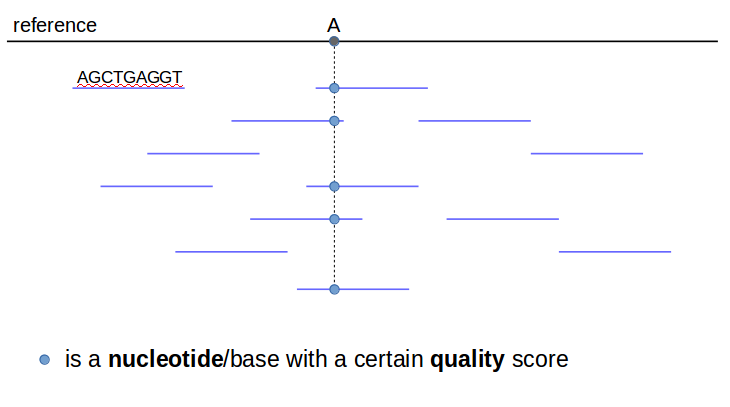
\includegraphics[scale=0.45]{Pics/mappedReads}
	\end{figure}

}

%%%%%%%%%%%%%%%%%%%%%%%%%%%%%%%%%%%%%%%%%%%%%%%%%%%%

\frame{\frametitle{Genotype likelihoods}

	\begin{block}{Likelihood}
		$P(D|G=\{A_1,A_2,...,A_n\})$
        \newline
		with
        \newline
		$A_i \in \{A,C,G,T\}$
        and $n$ being the ploidy
	\end{block}

How many genotypes likelihoods do we need to calculate for each each individual at each site?

}

%%%%%%%%%%%%%%%%%%%%%%%%%%%%%%%%%%%%%%%%%%%%%%%%%%%%

\frame{\frametitle{Genotype likelihoods}

	\begin{figure}
		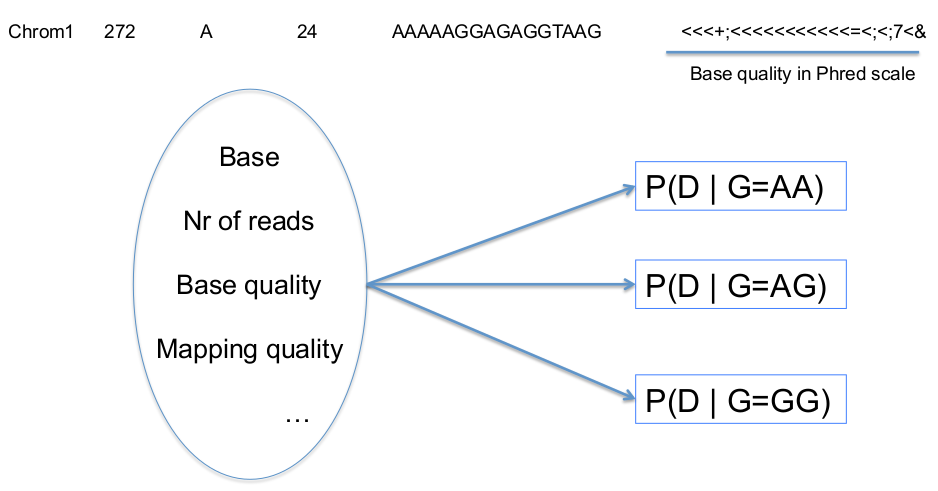
\includegraphics[scale=0.3]{Pics/genoLikes}
	\end{figure}

}


%%%%%%%%%%%%%%%%%%%%%%%%%%%%%%%%%%%%%%%%%%%%%%%%%%%%

\frame{\frametitle{Calculating genotype likelihoods}

\begin{block}{Likelihood function}

	\begin{equation*}
		P(D|G=\{A_1,A_2,...,A_N\}) = \prod_{i=1}^R \sum_{j=1}^N \frac{L_{A_j,i}}{N}
	\end{equation*}
 
 	\begin{itemize}
    	\item $L_{A_j,i} = P(D|A_G=A_j)$
    	\item $A_i \in \{A,C,G,T\}$
		\item $R$ is the depth (nr. of reads)
    	\item $N$ is the ploidy (nr. of chromosomes)
	\end{itemize}
    
\end{block}

Example:\\
AAAG, all with quality score equal to 20 (in phred score)\\
$P(D|G=AC) = ?$

}


%%%%%%%%%%%%%%%%%%%%%%%%%%%%%%%%%%%%%%%%%%%%%%%%%%%%

\frame{\frametitle{Calculating genotype likelihoods}

	\begin{block}{Likelihood function}

		\begin{equation*}
			P(D|G=\{A_1,A_2,...,A_N\}) = \prod_{i=1}^R \sum_{j=1}^N \frac{L_{A_j,i}}{N}
		\end{equation*}
  
	\end{block}

	\small{
	A\\
	A\\
	A\\
	G\\
	\& Q=20
	}

	\begin{equation*}
		P(D|G=\{A,C\}) = ...
	\end{equation*}

}

%%%%%%%%%%%%%%%%%%%%%%%%%%%%%%%%%%%%%%%%%%%%%%%%%%%%%%%%%%%%%%%%%%%%

\frame{\frametitle{Calculating genotype likelihoods}

	\begin{block}{Likelihood function}

		\begin{equation*}
			P(D|G=\{A_1,A_2,...,A_N\}) = \prod_{i=1}^R \sum_{j=1}^N \frac{L_{A_j,i}}{N}
		\end{equation*}
  
	\end{block}

	\small{
	A\\
	A\\
	A\\
	G\\ 
	\& Q=20
	}

	$N=2; i=1; A_1=A; A_2=C$

	\begin{equation*}
		P(D|G=\{A,C\}) = (\frac{L_{A,1}}{2} + \frac{L_{C,1}}{2}) \times ...
	\end{equation*}

	What are $L_{A,1}$ and $L_{C,1}$?

}

%%%%%%%%%%%%%%%%%%%%%%%%%%%%%%%%%%%%%%%%%%%%%%%%%%%%%%%%%%%%%%%%%%%%

\frame{\frametitle{Calculating genotype likelihoods}

	\begin{block}{Likelihood function}

		\begin{equation*}
			P(D|G=\{A_1,A_2,...,A_N\}) = \prod_{i=1}^R \sum_{j=1}^N \frac{L_{A_j,i}}{N}
		\end{equation*}
  
	\end{block}

	AAAG \& Q=20

	\begin{equation*}
			L_{C,1} = \frac{\epsilon}{3}	
	\end{equation*}

	\begin{equation*}
    	L_{A,1} = 1-\epsilon
	\end{equation*}
    
	\begin{equation*}
		P(D|G=\{A,C\}) = (\frac{1-\epsilon}{2} + \frac{\epsilon}{6}) \times ...
	\end{equation*}


}

%%%%%%%%%%%%%%%%%%%%%%%%%%%%%%%%%%%%%%%%%%%%%%%%%%%%%%%%%%%%%%%%%%%%

\frame{\frametitle{Calculating genotype likelihoods}

	\begin{block}{Likelihood function}

		\begin{equation*}
			P(D|G=\{A_1,A_2,...,A_N\}) = \prod_{i=1}^R \sum_{j=1}^N \frac{L_{A_j,i}}{N}
		\end{equation*}
  
	\end{block}

	AAAG \& Q=20

	\begin{equation*}
			L_{C,1} = \frac{\epsilon}{3}	
	\end{equation*}

	\begin{equation*}
    	L_{A,1} = 1-\epsilon
	\end{equation*}
    
	\begin{equation*}
		P(D|G=\{A,C\}) = (\frac{1-\epsilon}{2} + \frac{\epsilon}{6})^3  \times \frac{\epsilon}{3}
	\end{equation*}

	What is $\epsilon$?

}

%%%%%%%%%%%%%%%%%%%%%%%%%%%%%%%%%%%%%%%%%%%%%%%%%%%%%%%%%%%%%%%%%%%%

\frame{\frametitle{Calculating genotype likelihoods}

	\begin{columns}
	
    	\column{0.6\textwidth}   

		\begin{center}
			\begin{tabular}{c | c}
			Genotype & Likelihood (log10)\\
    		\hline
	    	AA & -2.49\\
    		\textbf{AC} & \textbf{-3.38}\\
    		AG & -1.22\\
    		AT & -3.38\\
        	CC & -9.91\\
      		CG & -7.74\\
        	CT & -9.91\\
         	GG & -7.44\\
          	GT & -7.74\\
        	TT & -9.91\\
        	\hline
			\end{tabular}
       	\end{center}

		\column{0.4\textwidth}

		A\\A\\A\\G\\$\epsilon=0.01$

	\end{columns}


}











% Genotype calling

\section{Genotype calling}

%%%%%%%%%%%%%%%%%%%%%%%%%%%%%%%%%%%%%%%%%%%%%%%%%%%

\frame{\frametitle{Genotype calling}

	\begin{columns}
	
    	\column{0.6\textwidth}   

		\begin{center}
			\begin{tabular}{c | c}
			Genotype & Likelihood (log10)\\
    		\hline
	    	AA & -2.49\\
    		AC & -3.38\\
    		AG & -1.22\\
    		AT & -3.38\\
            CC & -9.91\\
            CG & -7.74\\
            CT & -9.91\\
            GG & -7.44\\
            GT & -7.74\\
            TT & -9.91\\
        	\hline
			\end{tabular}
       	\end{center}

		\column{0.4\textwidth}

		AAAG \& $\epsilon=0.01$

		\begin{block}{}
			What is the genotype here?
		\end{block}

	\end{columns}


}

%%%%%%%%%%%%%%%%%%%%%%%%%%%%%%%%%%%%%%%%%%%%%%%%%%%

\frame{\frametitle{Genotype calling}

	\begin{columns}
	
    	\column{0.6\textwidth}   

		\begin{center}
			\begin{tabular}{c | c}
			Genotype & Likelihood (log10)\\
    		\hline
	    	AA & -2.49\\
    		AC & -3.38\\
    		\textbf{AG} & \textbf{-1.22}\\
    		AT & -3.38\\
            CC & -9.91\\
            CG & -7.74\\
            CT & -9.91\\
            GG & -7.44\\
            GT & -7.74\\
            TT & -9.91\\
        	\hline
			\end{tabular}
       	\end{center}

		\column{0.4\textwidth}

		AAAG \& $\epsilon=0.01$

		What is the genotype? AG.

		\begin{block}{Maximum Likelihood}
			The simplest genotype caller: choose the genotype with the highest likelihood.
		\end{block}

	\end{columns}


}

%%%%%%%%%%%%%%%%%%%%%%%%%%%%%%%%%%%%%%

\frame{\frametitle{Major and minor alleles}

	\begin{block}{Likelihood function}
		\begin{equation*}
			\log P(D|G=A) = \sum_{i=1}^R \log L_{A_j,i}
		\end{equation*}
	\end{block}

	AAAG \& $\epsilon=0.01$

	\begin{center}
		\begin{tabular}{c | c}
		Allele & Likelihood\\
    	\hline
	    \textbf{A} & \textbf{-2.49}\\
    	C & -3.38\\
    	\textbf{G} & \textbf{-1.22}\\
    	T & -3.38\\
        \hline
		\end{tabular}
	\end{center}

	We can reduce the genotype space to 3 entries (from 10).
    
}    
    
%%%%%%%%%%%%%%%%%%%%%%%%%%%%%%%%%%%%%%

\frame{\frametitle{Genotype calling}

	AAAG \& $\epsilon=0.01$ \& A,G alleles

	\begin{center}
		\begin{tabular}{c | c}
		Genotype & Likelihood\\
    	\hline
	    AA & -5.73\\
    	AG & -2.80\\
    	GG & -17.12\\
        \hline
		\end{tabular}
	\end{center}

	Examples varying qualities and reads...
    
}   

%%%%%%%%%%%%%%%%%%%%%%%%%%%%%%%%%%%%%%%%%%%

\frame{\frametitle{Genotype likelihood ratio}

	\begin{equation*}
		\log_{10} \frac{L_{G(1)}}{L_{G(2)}} > t
	\end{equation*}

	i.e. $t=1$ meaning that the most likely genotype is 10 times more likely than the second most likely one

	Pros and cons?
 	\begin{itemize}
 	\item Yes:
    \item No:
 	\end{itemize}

}

%%%%%%%%%%%%%%%%%%%%%%%%%%%%%%%%%%%%%%%%%%%

\frame{\frametitle{Genotype likelihood ratio}

	\begin{equation*}
		\log_{10} \frac{L_{G(1)}}{L_{G(2)}} > t
	\end{equation*}

	i.e. $t=1$ meaning that the most likely genotype is 10 times more likely than the second most likely one

	\begin{center}
		Pros and cons?
 		\begin{itemize}
 		\item Yes: genotype are called with higher \textbf{confidence}
    		\item No: more \textbf{missing} data
 		\end{itemize}
	\end{center}

}


%%%%%%%%%%%%%%%%%%%%%%%%%%%%%%%%%%%%%%%%%%%%%%%%%%%%%

\frame{
\frametitle{Statistical thinking}

\begin{figure}[!ht]
\centering
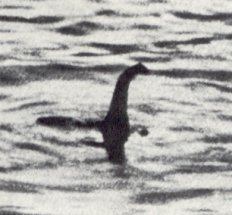
\includegraphics[width=4cm]{Pics/LochNessMonster.jpg}
\caption{Nessie, the Loch Ness Monster. True or fake?}
\end{figure}

}

%%%%%%%%%%%%%%%%%%%%%%%%%%%%%%%%%%%%%%%%%%%%%%%%%%%%%%%%

\frame{
\frametitle{Statistical thinking}

\begin{itemize}
\item $T = \{0,1\}$, whether I tell you I saw Nessie or not.
\item $N = \{0,1\}$, whether Nessie exists (I saw it) or not.
\end{itemize}

\begin{block}{Questions}
\begin{itemize}
\item What are $p(T=1|N=1)$ and $p(T=1|N=0)$?
\item What is a Maximum Likelihood Estimate of $N$?
\end{itemize}
\end{block}

}

%%%%%%%%%%%%%%%%%%%%%%%%%%%%%

\frame{
\frametitle{Statistical thinking}

Our inference on $N$ is driven solely by our observations, given by our likelihood function.

\begin{figure}[!ht]
\centering
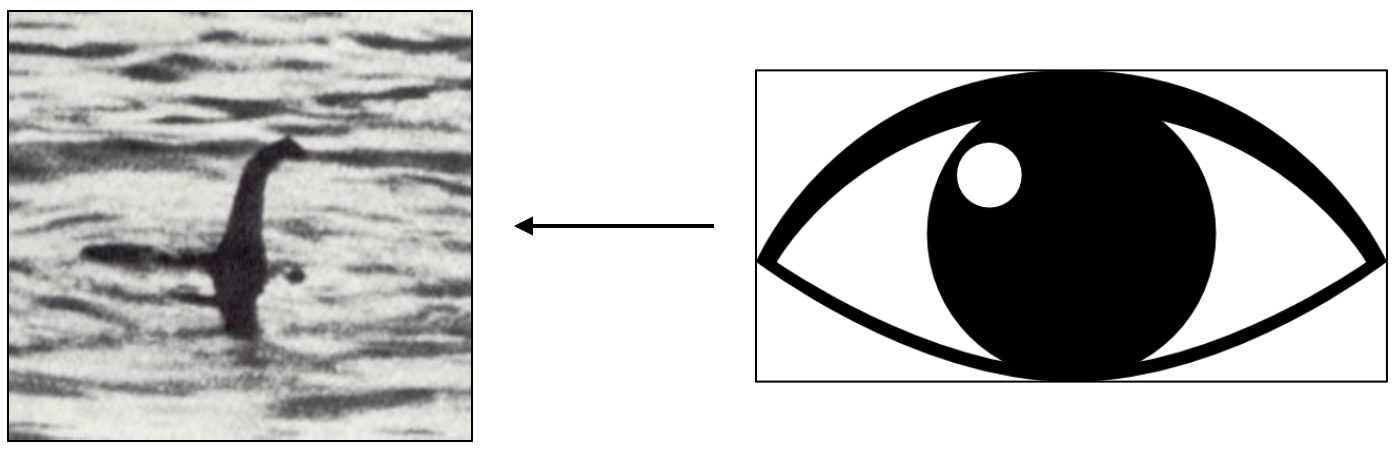
\includegraphics[width=5cm]{Pics/EyeOnly.png}
\caption{The eye: a "likelihood" organ.}
\end{figure}

}

%%%%%%%%%%%%%%%%%%%%%%%%%%%%%

\frame{
\frametitle{Statistical thinking}

In real life we take many decisions based not only on what we observe but also on some believes of ours.

\begin{figure}[!ht]
\centering
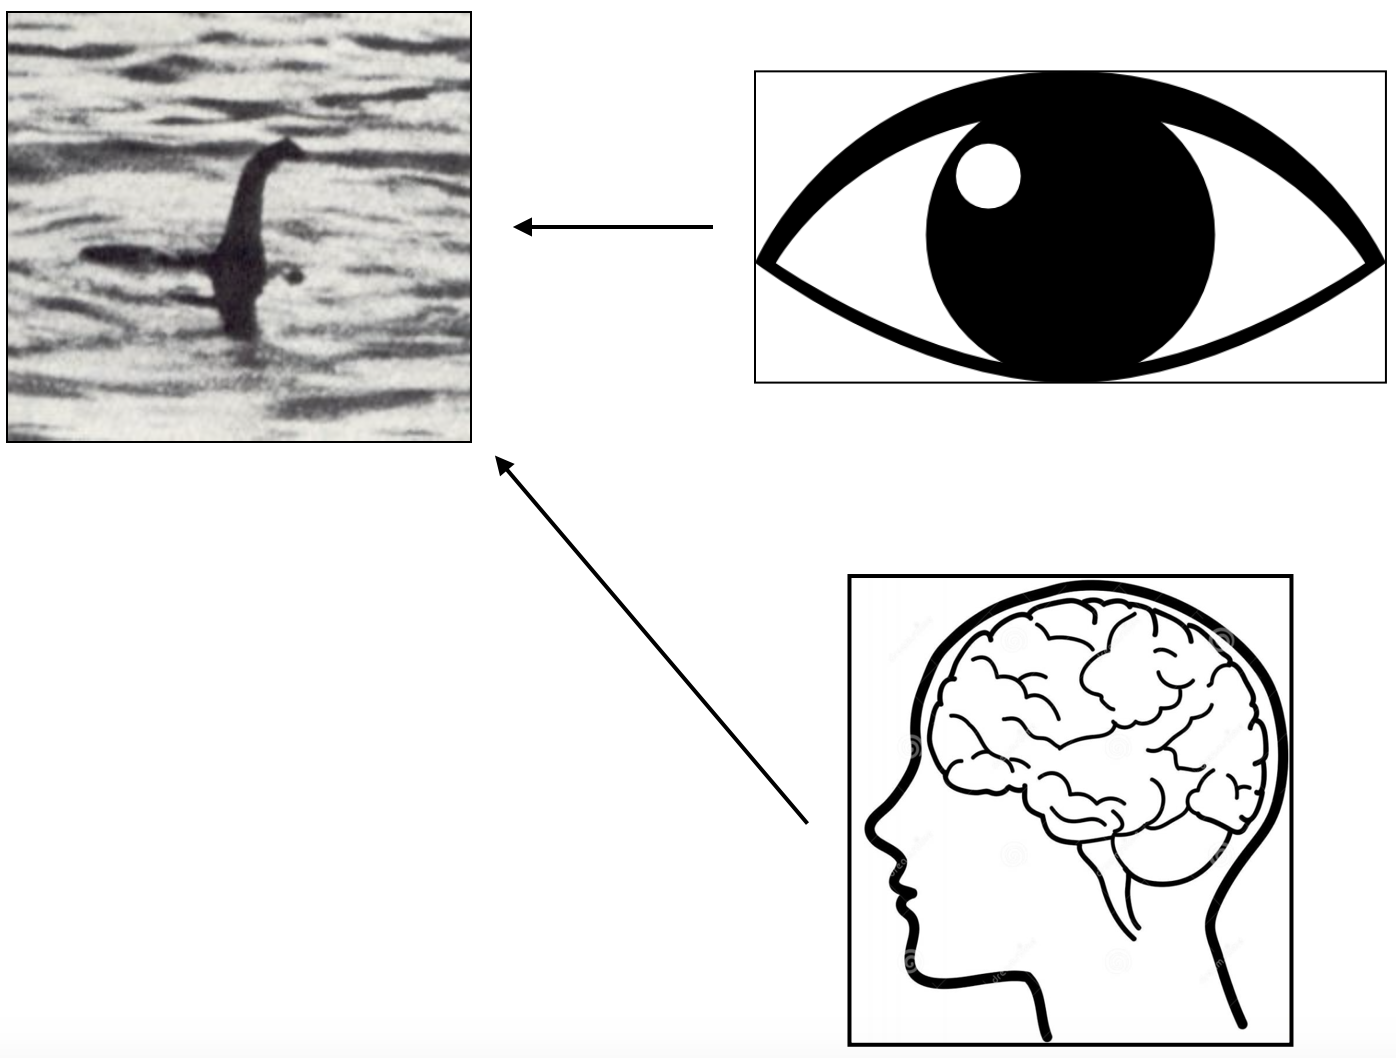
\includegraphics[width=5cm]{Pics/EyeBrain.png}
\caption{The brain: a "non-likelihood" organ.}
\label{Fig:EyeBrain}
\end{figure}

}

%%%%%%%%%%%%%%%%%%%%%%%%%%%%%%%%%%%%%%%%%%%%%%%%

\frame{
\frametitle{Bayesian thinking}

\begin{itemize}
\item with "eyes only" our intuition is that $p(N|T) \approx p(T|N)$
\item with "the brain" our intuition is that $p(N|T) \approx p(T|N)p(N)$
\end{itemize}

Our "belief" expresses the probability $p(N)$ \textbf{unconditional} of the data.

\begin{block}{Question}
How can we define $p(N)$?
\end{block}

}

%%%%%%%%%%%%%%%%%%%%%%%%%%%%%%%%%%%%%%%%%%%%%%%%%

\frame{
\frametitle{Bayesian thinking}

\begin{block}{}
The "belief" function $p(N)$ is called \textbf{prior probability} and the joint product of the likelihood $p(T|N)$ and the prior is proportional to the \textbf{posterior probability} $p(N|T)$.
\end{block}

\begin{block}{}
The use of posterior probabilities for inferences is called Bayesian statistics.
\end{block}

}

%%%%%%%%%%%%%%%%%%%%%%%%%%%%%%%%%%%%%%%%%%%%%%%%%

\frame{
\frametitle{Statistical inference}

If $D$ is the data and $\theta$ is your unknown parameter, then
\begin{itemize}
\item the frequentist conditions on parameters and integrates over the data, $p(D|\theta)$,
\item the Bayesian conditions on the data and integrates over the parameters, $p(\theta|D)$.
\end{itemize}

}

%%%%%%%%%%%%%%%%%%%%%%%%%%%%%%%%%%

\frame{
\frametitle{Statistical inference}

\begin{block}{Bayesian \textit{vs.} Likelihoodist}
\begin{itemize}
\item we derive "proper" probability distributions of our parameters rather than deriving a point estimate;
\item a probability is assigned to a hypothesis rather than a hypothesis is tested;
\item we can "accept" the null hypothesis rather than "fail to reject" it;
\item parsimony imposed in model choice rather than correcting for multiple tests.
\end{itemize}
\end{block}

}

%%%%%%%%%%%%%%%%%%%%%%%%%%%%%%%%%%%%%%%%

\frame{
\frametitle{Bayesian inference}

\begin{figure}[!ht]
\centering
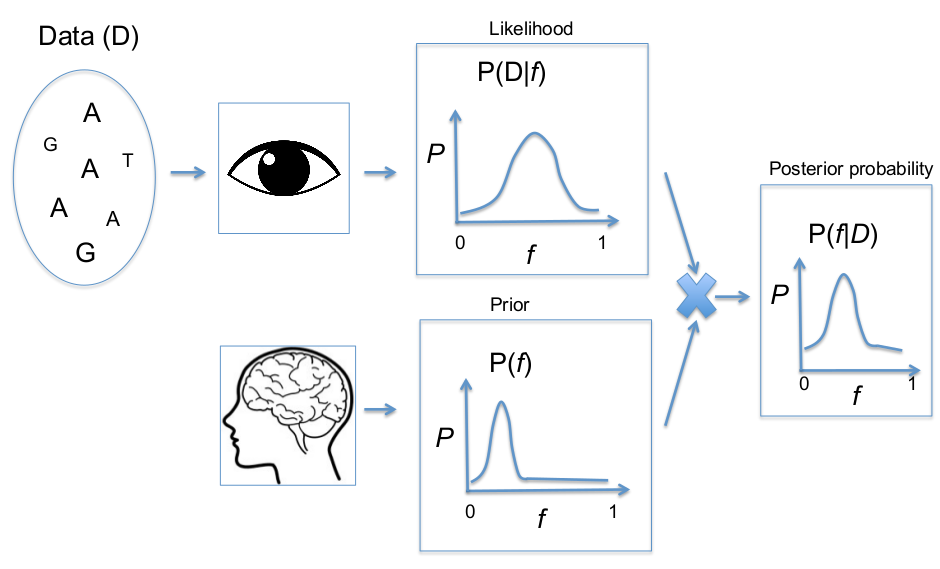
\includegraphics[width=8cm]{Pics/bayesian.png}
\end{figure}

}


%%%%%%%%%%%%%%%%%%%%%%%%%%%%%%

\frame{
\frametitle{Bayesian concepts}

\begin{block}{Bayes' Theorem}

\begin{equation}
p(\vec{\theta}|\vec{y}) = \frac{f(\vec{y}|\vec{\theta})\pi(\vec{\theta})}{m(\vec{y})} = \frac{f(\vec{y}|\vec{\theta})\pi(\vec{\theta})}{\int f(\vec{y}|\vec{\theta}) d\vec{\theta}}
\end{equation}
\end{block}

\begin{itemize}
\item $\vec{\theta}$ is not a fixed parameter but a random quantity with prior distribution $\pi(\vec{\theta})$
\item $p(\vec{\theta}|\vec{y})$ is the posterior probability distribution of $\vec{\theta}$
\item $\int p(\vec{\theta}|\vec{y})d\vec{\theta}=1$
\end{itemize}

}

%%%%%%%%%%%%%%%%%%%%%%%%%%%%%%%%%%%%%%%%%%%%%

\frame{
\frametitle{Genotype posterior probability}

	AAAG \& $\epsilon=0.01$ \& A,G alleles

	\begin{center}
		\begin{tabular}{c | c | c | c}
		Genotype & Likelihood (log) & Prior & Posterior\\
    	\hline
	    AA & -5.73 &  & \\
    	AG & -2.80 &  & \\
    	GG & -17.12 &  & \\
        \hline
		\end{tabular}
	\end{center}


}

%%%%%%%%%%%%%%%%%%%%%%%%%%%%%%%%%%%%%%%%%%%%%

\frame{
\frametitle{Genotype posterior probability}

	AAAG \& $\epsilon=0.01$ \& A,G alleles

	\begin{center}
		\begin{tabular}{c | c | c | c}
		Genotype & Likelihood (log) & Prior & Posterior\\
    	\hline
	    AA & -5.73 & 1/3 & 0.05\\
    	AG & -2.80 & 1/3 & 0.95\\
    	GG & -17.12 & 1/3 & ~0\\
        \hline
		\end{tabular}
	\end{center}

	Only call genotypes if the largest probability is above a certain threshold (e.g. 0.95).

}

%%%%%%%%%%%%%%%%%%%%%%%%%%%%%%%%%%%%%%%%%%%%%%%%%

\frame{
\frametitle{Genotype posterior probability}

	AAAG \& $\epsilon=0.01$ \& A,G alleles \& \textbf{A is the reference allele}

	$P(AA) > P(AG) > P(GG)$

	\begin{center}
		\begin{tabular}{c | c | c | c}
		Genotype & Likelihood (log) & Prior & Posterior\\
    	\hline
	    AA & -5.73 & 0.80 & 0.22\\
    	AG & -2.80 & 0.15 & 0.78\\
    	GG & -17.12 & 0.05 & ~0\\
        \hline
		\end{tabular}
	\end{center}
    

	The reference allele is just one of the possible alleles, often chosen arbitrarily: why give it so much weight?

}

%%%%%%%%%%%%%%%%%%%%%%%%%%%%%%%%%%%%%%%%%%%%%%%%%

\frame{
\frametitle{Genotype posterior probability}

	AAAG \& $\epsilon=0.01$ \& A,G alleles \& \textbf{$f(A)=0.7$} from a reference panel

	$P(AA)=?$;
	$P(AG)=?$;
    	$P(GG)=?$

	\begin{center}
		\begin{tabular}{c | c | c | c}
		Genotype & Likelihood (log) & Prior & Posterior\\
    	\hline
	AA & -5.73 &  & \\
    	AG & -2.80 &  & \\
    	GG & -17.12 &  & \\
        \hline
		\end{tabular}
	\end{center}

}

%%%%%%%%%%%%%%%%%%%%%%%%%%%%%%%%%%%%%%%%%%%%%%%%%

\frame{
\frametitle{Genotype posterior probability}

        AAAG \& $\epsilon=0.01$ \& A,G alleles \& \textbf{$f(A)=0.7$} from a reference panel

        $P(AA)=?$;
    $P(AG)=?$;
    $P(GG)=?$

        \begin{center}
                \begin{tabular}{c | c | c | c}
                Genotype & Likelihood (log) & Prior & Posterior\\
        \hline
            AA & -5.73 & 0.49 & 0.06\\
        AG & -2.80 & 0.42 & 0.94\\
        GG & -17.12 & 0.09 & ~0\\
        \hline
                \end{tabular}
        \end{center}

        If the assumption of HWE can be reasonably met.

}

%%%%%%%%%%%%%%%%%%%%%%%%%%%%%%%%%%%%%%%%%%%%%%%%%


\frame{\frametitle{Empirical Bayesian inference}

\begin{figure}[!ht]
\centering
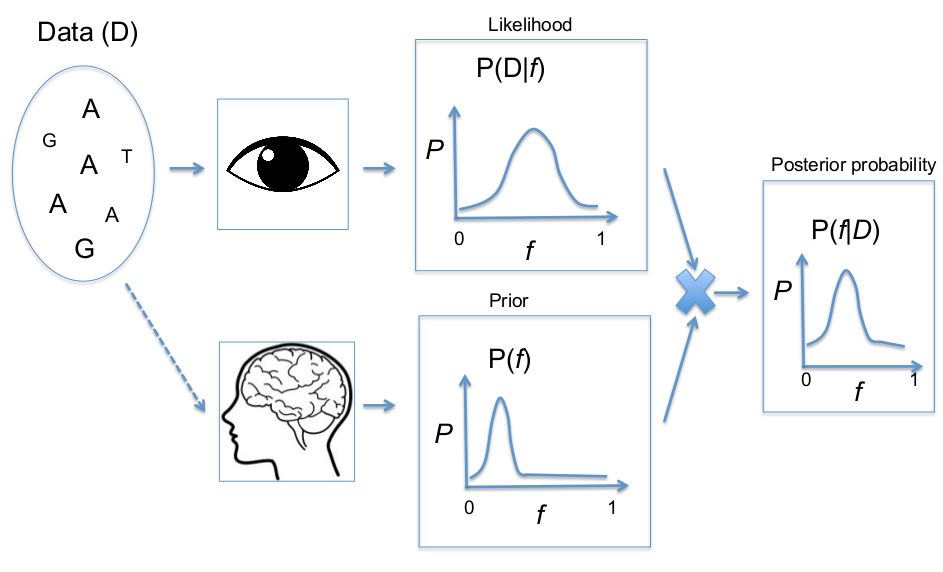
\includegraphics[width=8cm]{Pics/statEB.png}
\end{figure}



}

%%%%%%%%%%%%%%%%%%%%%%%%%%%%%%%%%%%%%%%%%%%%%%%%%

\frame{\frametitle{Genotype posterior probability}

	AAAG \& $\epsilon=0.01$ \& A,G alleles \& \textbf{$f(A)=0.6$} from the data itself

	$P(AA)=?$;
    $P(AG)=?$;
    $P(GG)=?$

	\begin{center}
		\begin{tabular}{c | c | c | c}
		Genotype & Likelihood (log) & Prior & Posterior\\
    	\hline
	    AA & -5.73 & 0.49 & 0.04\\
    	AG & -2.80 & 0.42 & 0.96\\
    	GG & -17.12 & 0.09 & ~0\\
        \hline
		\end{tabular}
	\end{center}

	\begin{itemize}
	\item if the assumption of HWE can be reasonably met
    \item if you have enough samples to have a robust estimate of the allele frequencies
	\end{itemize}

	How can we estimate allele frequencies?
	

}




% Allele frequencies and SNP calling

\section{SNP calling}

%%%%%%%%%%%%%%%%%%%%%%%%%%%%%%%%%%%%%%%%%%%%%%%%%%%%%%%

\frame{
\frametitle{SNP calling procedures}

	\begin{figure}[!ht]
	\centering
	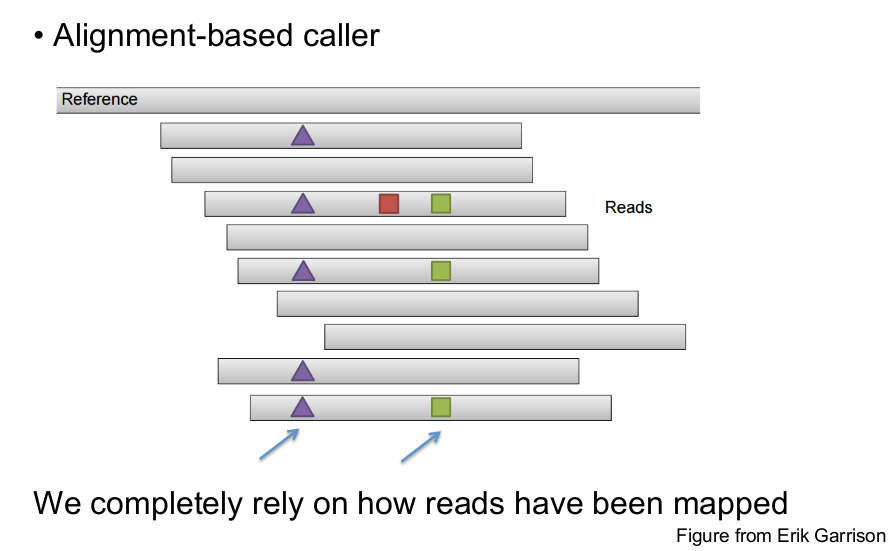
\includegraphics[width=9cm]{Pics/snp1.png}
	\end{figure}

}

%%%%%%%%%%%%%%%%%%%%%%%%%%%%%%%%%%%%%%%%%%%%%%%%%%%%%%%

\frame{
\frametitle{SNP calling procedures}

	\begin{figure}[!ht]
	\centering
	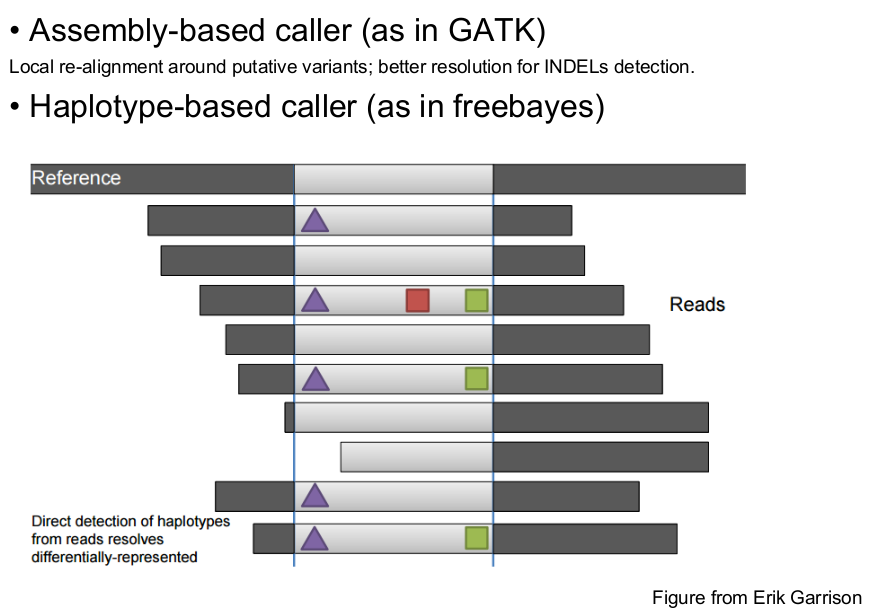
\includegraphics[width=9cm]{Pics/snp2.png}
	\end{figure}

}

%%%%%%%%%%%%%%%%%%%%%%%%%%%%%%%%%%%%%%%%%%%%%%%%%%%%%%%%%%

\frame{
\frametitle{Estimating allele frequencies}

	Assuming 2 alleles (A,G) with true allele frequency of 0.50

	\begin{center}
	\begin{tabular}{c|c|c|c}
	Sample & True genotype & Reads allele A & Read allele G\\
    \hline
    1 & AA & 7 & 0\\
    2 & AA & 25 & 1\\
    3 & AG & 5 & 3\\
    4 & AG & 4 & 4\\
    5 & GG & 0 & 2\\
    6 & GG & 0 & 4\\
    \hline
	\end{tabular}	
	\end{center}

	What is the simplest estimator of allele frequencies?

}


%%%%%%%%%%%%%%%%%%%%%%%%%%%%%%%%%%%%%%%%%%%%%%%%%%%%%%%%%%

\frame{
\frametitle{Estimating allele frequencies}

	Assuming 2 alleles (A,G) with true allele frequency of 0.50

	\begin{center}
	\begin{tabular}{c|c|c|c}
	Sample & True genotype & Reads allele A & Read allele G\\
    \hline
    1 & AA & 7 & 0\\
    2 & AA & 25 & 1\\
    3 & AG & 5 & 3\\
    4 & AG & 4 & 4\\
    5 & GG & 0 & 2\\
    6 & GG & 0 & 4\\
    \hline
    Total & & 41 & 14\\
    \hline
	\end{tabular}
	\end{center}

	\begin{equation*}
		\hat{f} = \frac{\sum_{i=1}^N n_{A,i}}{ \sum_{i=1}^N (n_{A,i}+n_{G,i}) }
	\end{equation*}

	$\hat{f}=0.75$

	What is wrong with this estimator?

}

%%%%%%%%%%%%%%%%%%%%%%%%%%%%%%%%%%%%%%%%%%%%%%%%%%%%%%%%%%

\frame{
\frametitle{Estimating allele frequencies}

	Assuming 2 alleles (A,G) with true allele frequency of 0.50

	\begin{center}
	\begin{tabular}{c|c|c|c}
	Sample & True genotype & Reads allele A & Read allele G\\
    \hline
    1 & AA & 7 & 0\\
    2 & AA & 25 & 1\\
    3 & AG & 5 & 3\\
    4 & AG & 4 & 4\\
    5 & GG & 0 & 2\\
    6 & GG & 0 & 4\\
    \hline
    Total & & 41 & 14\\
    \hline
	\end{tabular}
	\end{center}
    
    \begin{equation*}
		\hat{n_A} = \sum_{i=1}^N (1-\epsilon)n_{A,i} + \epsilon n_{G,i} - \epsilon n_{A,i} - (1-\epsilon)n_{G,i} = \sum_{i=1}^N (1-\epsilon)(n_{A,i}-n_{G,i}) + \epsilon(n_{G,i}-n_{A,i})
	\end{equation*}
    
    $\hat{f}=0.77$
}


%%%%%%%%%%%%%%%%%%%%%%%%%%%%%%%%%%%%%%%%%%%%%%%%%%%%%%%%%%

\frame{
\frametitle{Estimating allele frequencies}

	\begin{block}{Maximum Likelihood estimator}
		\begin{equation*}
			P(D|f) = \prod_{i=1}^N \sum_{g \in \{0,1,2\}} P(D|G=g) P(G=g,f)
		\end{equation*}
	\end{block}

	$P(D|G=g)$ is the genotype likelihood and $P(G=g,f)$ is given by HWE (for instance).

	In our previous example, $\hat{f}=0.46$ much closer to the true value than previous estimators.

}

%%%%%%%%%%%%%%%%%%%%%%%%%%%%%%%%%%%%%%%%%%%%%%%%%%%%%%%%%%%%%

\frame{
\frametitle{SNP calling}

	\begin{block}{Challenges}
	\begin{itemize}
	\item If high levels of missing data, then genotypes can be lost.
    \item Rare variants are hard to detect.
    \item Trade off between false positive and false negative rates.
	\end{itemize}
	\end{block}

	\begin{block}{How to call SNPs?}
	\begin{itemize}
	\item If at least one heterozygous genotype has been called.
    \item If the estimated allele frequency is above a certain threshold.
	\end{itemize}
	\end{block}


}


%%%%%%%%%%%%%%%%%%%%%%%%%%%%%%%%%%%%%%%%%%%%%%%%%%%%%%%%%%%%%

\frame{
\frametitle{SNP calling}

Call a SNP if
\begin{equation*}
	\hat{f} \geq t
\end{equation*}
where $t$ can be the minimum sample allele frequency detectable (e.g. $t=1/2N$ with $N$ diploids).

}


%%%%%%%%%%%%%%%%%%%%%%%%%%%%%%%%%%%%%%%%%%%%%%%%%%%%%%%%%%%%%

\frame{
\frametitle{Likelihood Ratio Test}

A Likelihood Ratio Test (LRT) compares the goodness	of fit between the null and the alternative model:
\begin{itemize}
\item Null model: $f=0$
\item Alternative model: $f \neq 0$
\end{itemize}

\begin{equation*}
T = -2 \log \frac{L(f=0)}{L(f=\hat{f}_{MLE})}
\end{equation*}

where $T$ is $\chi^2$ distributed with 1 degree of freedom.

}







%%%%%%%%%%%%%%%%%%%%%%%%%%%%%%%%%%%%%%%%%%%%%%%%%%%%%%%%%

% SCRATCH

\section*{ }
\frame{
 	\vbox{}
% 	\vfill
	\begin{centering}
	{\LARGE \usebeamercolor[fg]{title} Thank you for your attention}
	\par
	\end{centering}
}

\end{document}